\subsection{State machine}

\begin{figure}
  \begin{center}
    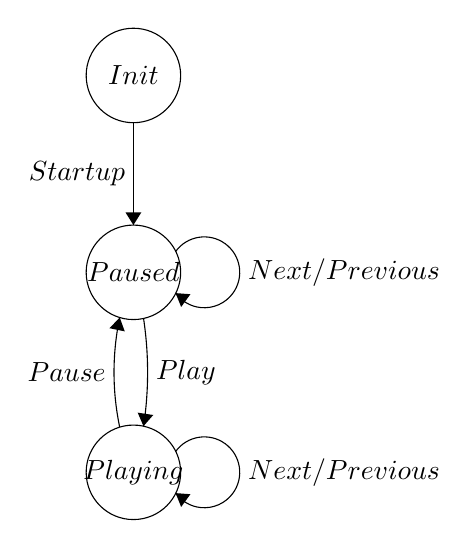
\begin{tikzpicture}[scale=0.2]
      \tikzstyle{every node}+=[inner sep=0pt]
      \draw [black] (36.9,-11.6) circle (3);
      \draw (36.9,-11.6) node {$Init$};
      \draw [black] (36.9,-24.1) circle (3);
      \draw (36.9,-24.1) node {$Paused$};
      \draw [black] (36.9,-36.8) circle (3);
      \draw (36.9,-36.8) node {$Playing$};
      \draw [black] (36.9,-14.6) -- (36.9,-21.1);
      \fill [black] (36.9,-21.1) -- (37.4,-20.3) -- (36.4,-20.3);
      \draw (36.4,-17.85) node [left] {$Startup$};
      \draw [black] (37.543,-27.028) arc (8.61666:-8.61666:22.839);
      \fill [black] (37.54,-33.87) -- (38.16,-33.16) -- (37.17,-33.01);
      \draw (38.3,-30.45) node [right] {$Play$};
      \draw [black] (39.58,-22.777) arc (144:-144:2.25);
      \draw (44.15,-24.1) node [right] {$Next/Previous$};
      \fill [black] (39.58,-25.42) -- (39.93,-26.3) -- (40.52,-25.49);
      \draw [black] (39.58,-35.477) arc (144:-144:2.25);
      \draw (44.15,-36.8) node [right] {$Next/Previous$};
      \fill [black] (39.58,-38.12) -- (39.93,-39) -- (40.52,-38.19);
      \draw [black] (36.029,-33.933) arc (-168.15785:-191.84215:16.974);
      \fill [black] (36.03,-26.97) -- (35.38,-27.65) -- (36.35,-27.85);
      \draw (35.17,-30.45) node [left] {$Pause$};
    \end{tikzpicture}
  \end{center}
  \caption{The state machine that controls the system}
  \label{fig:fsm}
\end{figure}

The overall system is driven by a finite state machine, shown in figure
\ref{fig:fsm}. Using a state machine to control the system allowed for a clean
implementation of complex logic, where alternative solutions would quickly
become unmaintainable.  Also to further maintainability, the state machine
operates asynchronously of the events it reacts to. Interrupts generate events
that are posted to a queue, and the state machine reads from the queue when the
controller wakes up from sleep. This allows for quick return from interrupt
service routines, which is a desirable feature. As it is more easily
extensible, an implementation based on a table of function pointers was chosen
for the state machine.
